\chapter{Fundamentals}
\label{chap:refs}

Under the term \emph{ray tracing} we understand the utilization of algorithms that involve the casting of virtual light rays for generating images. The purpose of these light rays is to archive high visual realism by approximating real-life behavior \todo{is that right?}. The reason we are able to perceive nearby objects or persons is due to the fact that light, which is being emitted from light sources, either natural or artificial, is interacting with these objects or persons, it is being reflected off by their surfaces towards our vision sensory organs after possibly being reflected a multiple times before from other surfaces. \todo{what?}
The purpose of ray tracing algorithms is to imitate this behavior, usually by tracing these light rays in reverse order from the sensory organs (or a virtual camera or an "eye point") back to the emitting light source.

\begin{figure}[h]
	\centering
	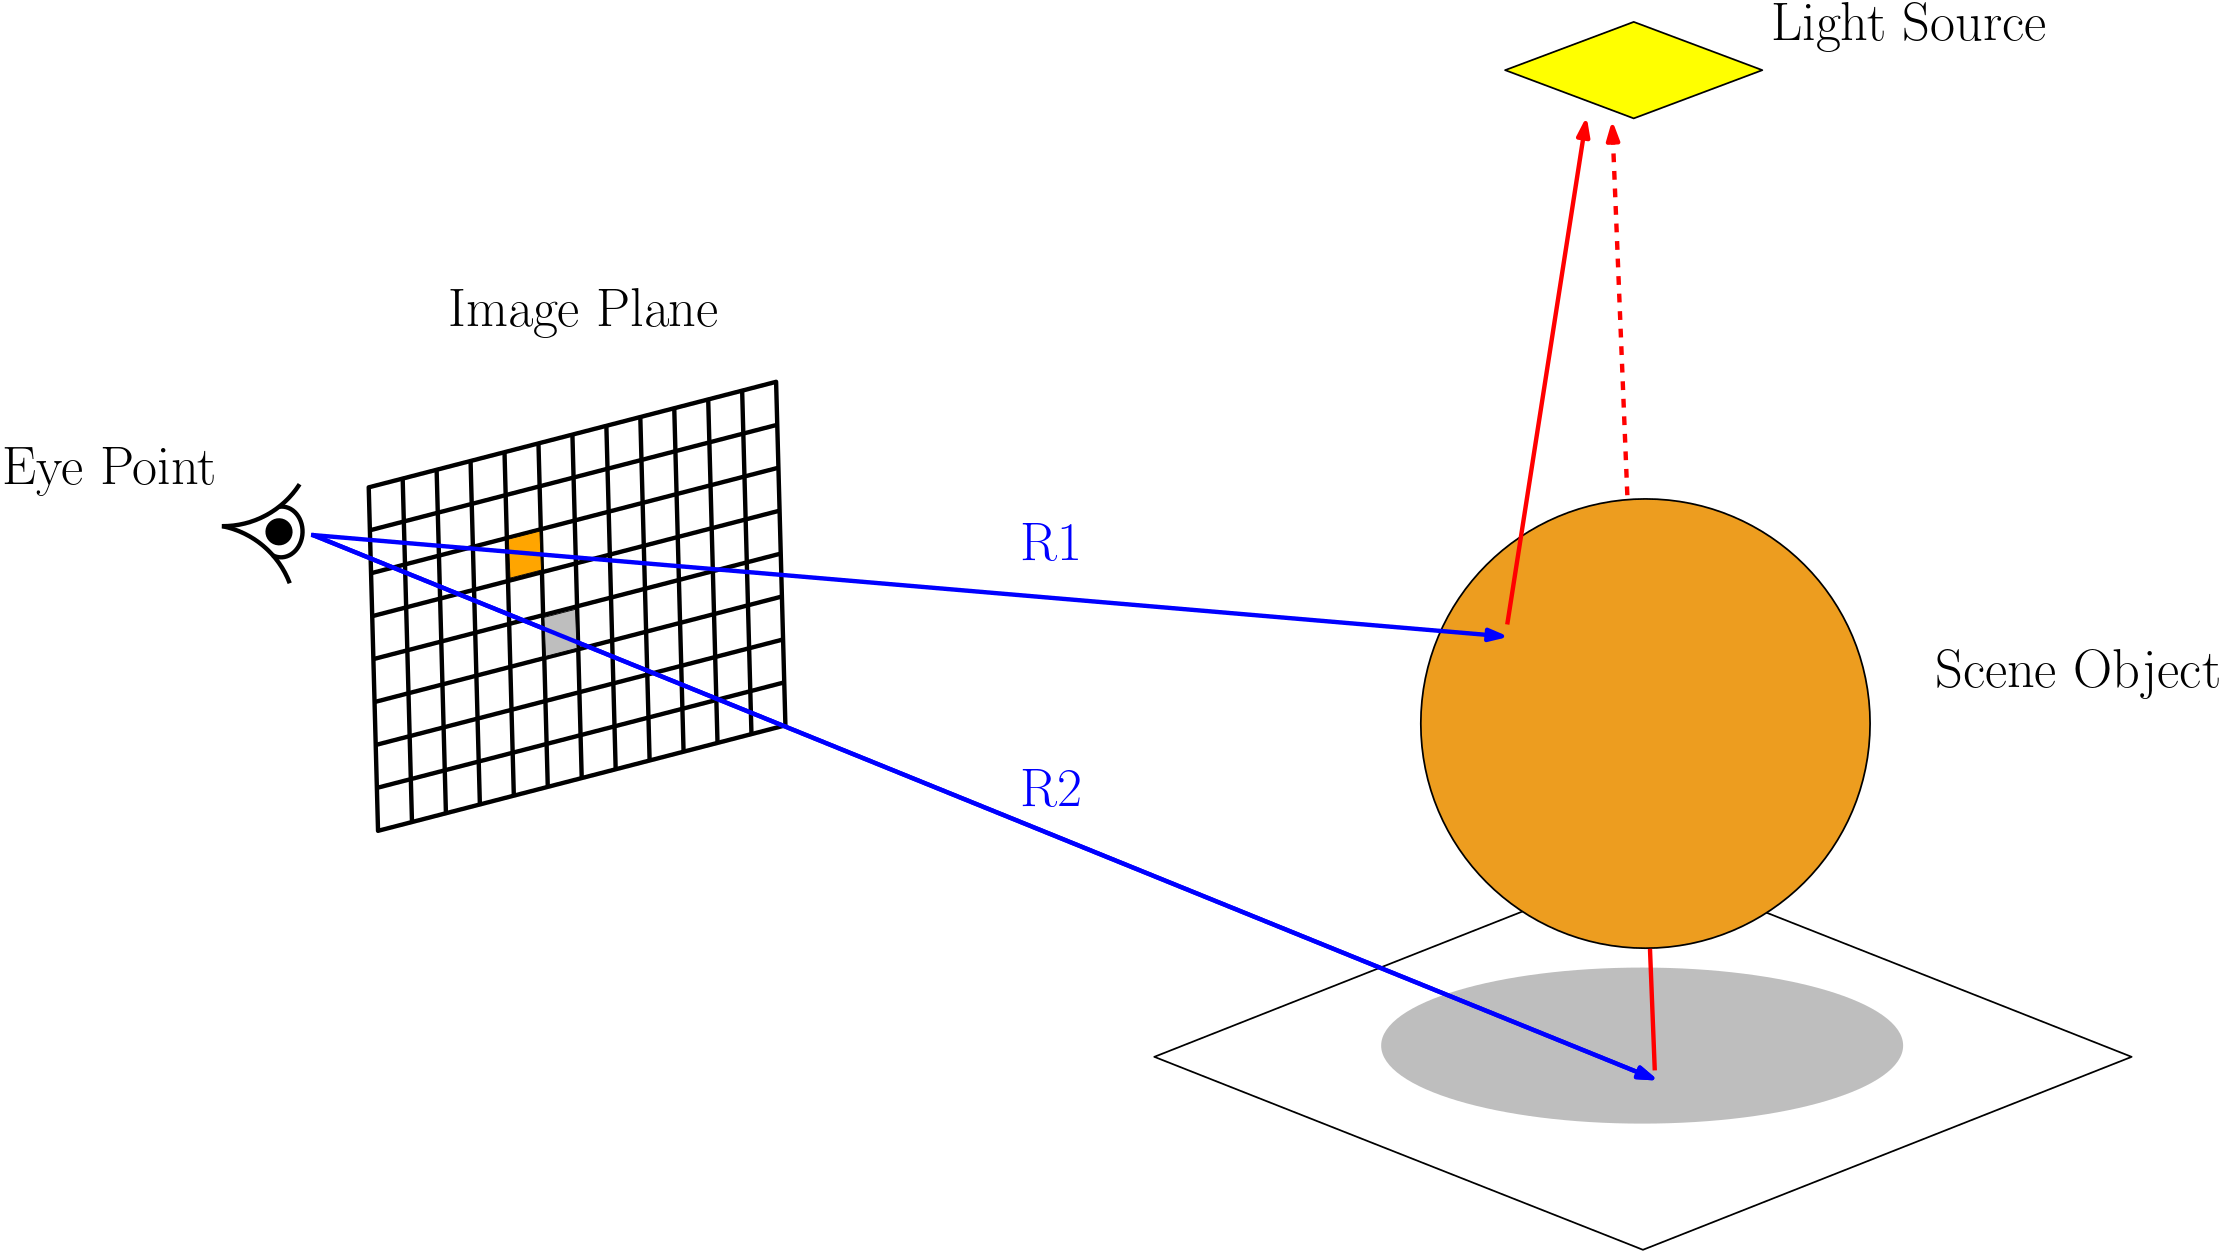
\includegraphics[width=.9\linewidth]{img/1 fundamentals/ray_tracing.png}
	\caption{Ray tracing procedure for calculating global illuminate.}
	\label{fig:raytracer_general}
\end{figure}

An advantage of these ray tracing algorithms is that the core procedure is straightforward when viewed from a theoretical point of view. Figure \ref{fig:raytracer_general} shows an example of a virtual scene. It consists of an orange sphere, a white ground plane, and a plane acting as an area light source. Furthermore, there exists an image plane on which the 2D image of the 3D scene will be projected. A ray is consisting of two components, an origin point and a direction vector. The "Eye Point" in \ref{fig:raytracer_general} will serve as the origin of the cast rays (sometimes, the Eye Point is referred to as Camera or Virtual Camera). In the figure, the image plane is composed of multiple quadratic "cells" that represent the actual pixels of the resulting image. Through each of these cells, a ray is cast into the scene from the eye point. The next step is to determine, whether that ray hit a particular geometry by performing intersection tests on all geometries in the scene. In case a geometry is hit, a secondary ray is generated with its origin at the intersection point and its direction toward the light source. In case this secondary light ray does not intersect any other geometry between its origin and the light source, this means that the first intersection point is exposed to light and the material color at that point is used for the corresponding pixel (see R1 in figure \ref{fig:raytracer_general}). Otherwise, the intersection point must be in shadow (see R2). This procedure generates an image with local illumination.

The following chapter is dedicated to providing background information on ray tracing, shape representation in rendering systems, and ray acceleration data structures. Furthermore, the Embree framework is introduced. \todo{maybe rephrase}

\section{Ray Tracing Algorithms}


\subsection{Origins of Ray Tracing}
As briefly mentioned in the Introduction, ray tracing was pioneered in 1968 by \cite{appel1968some}. The aim of his work was to provide basic shading for line drawings yielding a better communication of spatial relation and depth of objects in the rendered image.

\begin{figure}[h]
	\centering
	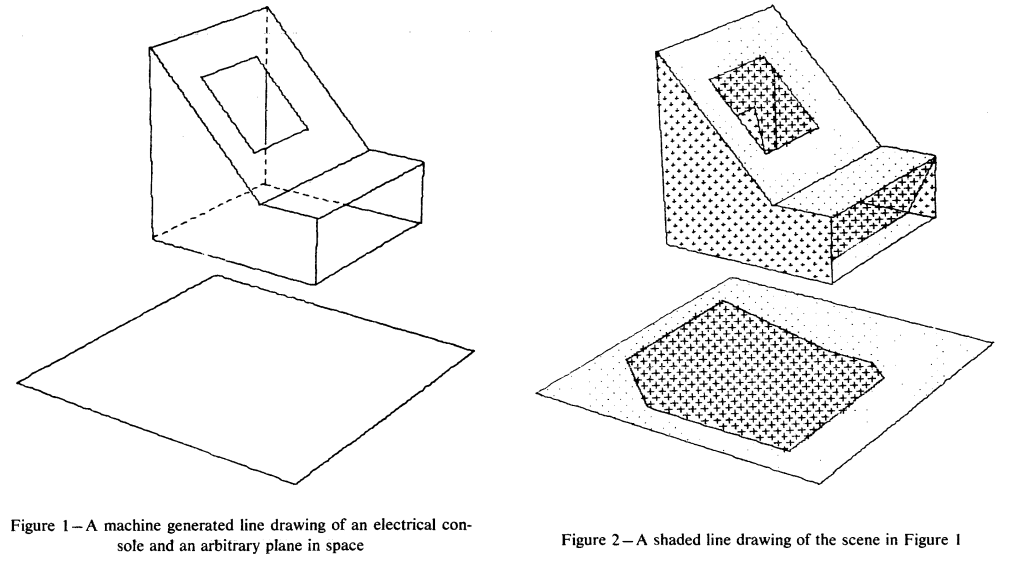
\includegraphics[width=1\linewidth]{img/1 fundamentals/appel_comp}
	\caption{Figures from \cite{appel1968some}. Left figure shows plain solid geometry and right figure shows the same solid with shading applied to it.}
	\label{fig:appel}
\end{figure}
\todo{can I use figures from other papers?}

Figure \ref{fig:appel} demonstrates this: without the additional shading information, it would be difficult for the observer to perceive the position of the upper geometry relative to the plane.

In order to achieve this shading, virtual light rays are shot from a scene light source in random directions. Whenever one such ray intersects a geometry, a character or symbol (e.g. a "plus"-symbol or small square) is placed at that intersection point. If enough such rays would be cast, areas on the solid that are exposed to light would be shaded by these symbols.
The result would then come to be by inverting the shaded and non-shaded areas of the geometry.

The intensity of light $I$ incident to the light source is described by the following equation:

\begin{equation}
I = S\frac{\cos{\theta}}{{D}^2}
\end{equation}

where $S$ is the intensity of the light source, $\cos{\theta}$ the angle between the ray and the surface normal at the intersection point and $D$ the distance between intersection point and light source.

In order to achieve convincing results, a high number of rays had to be generated ("Even for about 1000 light rays results were splotchy." \cite[p 3]{appel1968some}). At the time of publication, computational power of hardware could hardly be used for this.

The idea of casting rays later became a key utilization for a shading model that aimed for higher realism by taking the "global setting" of geometries into account \cite{whitted1979improved}. A variety of shading models existed at that time, which were able to convincingly display optical effects. However, these models usually worked only in special cases and not well with each other, as noted by Andrew Glassner in the preface of his book \citetitle{glassner1989introduction} \cite{glassner1989introduction}. \todo{is this good?} Some models existed that were good at calculating reflection effects, but could not handle refraction effects well. And vice versa. 

\cite{whitted1979improved} introduced a shading model that would truthfully simulate reflection, shadows and refraction as well as the effects of other conventional shading models at that time.  

The model is partially derived from an empirical reflection model developed by \cite{phong1975illumination}, which assumes that light, which is reflected from a surface, is composed by three types of reflection: ambient reflection, diffuse reflection and specular reflection. The following equation describes this model:

\begin{equation} \label{eq:phong}
I = k_{a} + k_{d}\sum_{j}(n*L_{j}) + k_{s}\sum_{j}(n*L_{j}\prime)^{\alpha}
\end{equation}

\noindent where
\begin{description}
	\setlength\itemsep{0.05em}
	\item  [$I$] is the reflected intensity
	\item  [$I_{a}$] is the ambient reflection coefficient
	\item  [$k_{d}$] is the diffuse reflection coefficient
	\item  [$k_{s}$] is the specular reflection coefficient
	\item  [$n$] is the unit surface normal at an intersection point
	\item  [$L_{j}$] is a vector in the direction of the $j$th light source
	\item  [$L_{j}\prime$] is a half vector between the eye point and the $j$th light source, and
	\item  [$\alpha$] is the glossiness coefficient.
\end{description}

This model even nowadays finds popularity among real time graphics due to its low computational cost and convincing (although not physically plausible) results. \todo{maybe reformulate}
The model assumes furthermore that light sources are located at an infinite distance from the scene geometry, and thus, it does not account for objects within the scene acting as light sources. It was observed in \cite{newell1977progression}, \todo{verify this} that this can critically affect the specular reflection component of Equation \ref{eq:phong}.

\begin{figure}[h]
	\centering
	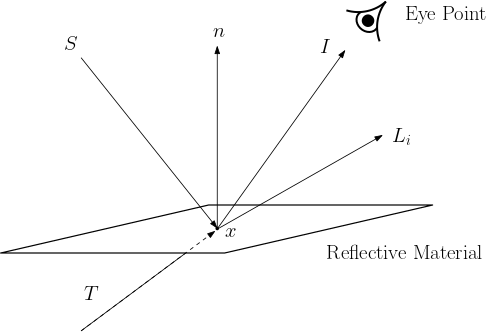
\includegraphics[width=.7\linewidth]{img/1 fundamentals/whitted.png}
	\caption{Light intensity propagated towards an observer being composed of a specular reflection component $S$ and a transmissive reflection component $T$.}
	\label{fig:whitted_model}
\end{figure}

As opposed to the Phong shading model, Whitted's model assumes that the light intensity $I$ arriving at the $Eye Point$ from the intersection point $x$ along the outgoing direction $\omega_{o}$ is conglomerated by a specular reflection component $S$, being propagated along direction $\omega_{s}$ and a transmission component $T$, being propagated along direction $\omega_{t}$. This is shown in Figure \ref{fig:whitted_model}.
The model is given by the equation:
\begin{equation} \label{eq:whitted}
I = k_{a} + k_{d}\sum_{j}(n*L_{j}) + k_{s}S + k_{t}T
\end{equation}

\noindent where
\begin{description}
	\setlength\itemsep{0.05em}
	\item  $S$ is the light intensity of the specular reflection
	\item  $T$ is the light intensity of the transmission, and
	\item  $k_{s}$ is the transmission coefficient
\end{description}
The ambient and diffuse term are maintained from Equation \ref{eq:phong}. 

The model is capable of generating images with a high degree of realism, preconditioned that the coefficients of equation \ref{eq:whitted} are reasonably chosen. Whitted noted in his paper that "for the best
accuracy they [the coefficients] should be functions that incorporate an
approximation of the Fresnel reflection". 
Generally, Equation \ref{eq:whitted} approximates the reflection of light towards an observer (or camera, or "Eye Point") from a single surface. However, in nature, light that is propagated towards a viewer from a surface most certainly has interacted with other surfaces before. If true realism of computer generated images is desired, this fact has to be taken into consideration, even for virtual scenes with moderately complex geometry. An example of such an event can be seen in Figure \ref{fig:whitted_rays}.

\begin{figure}[h]
	\centering
	\subfloat[Light is reflected from other surfaces before reaching the Eye Point.]{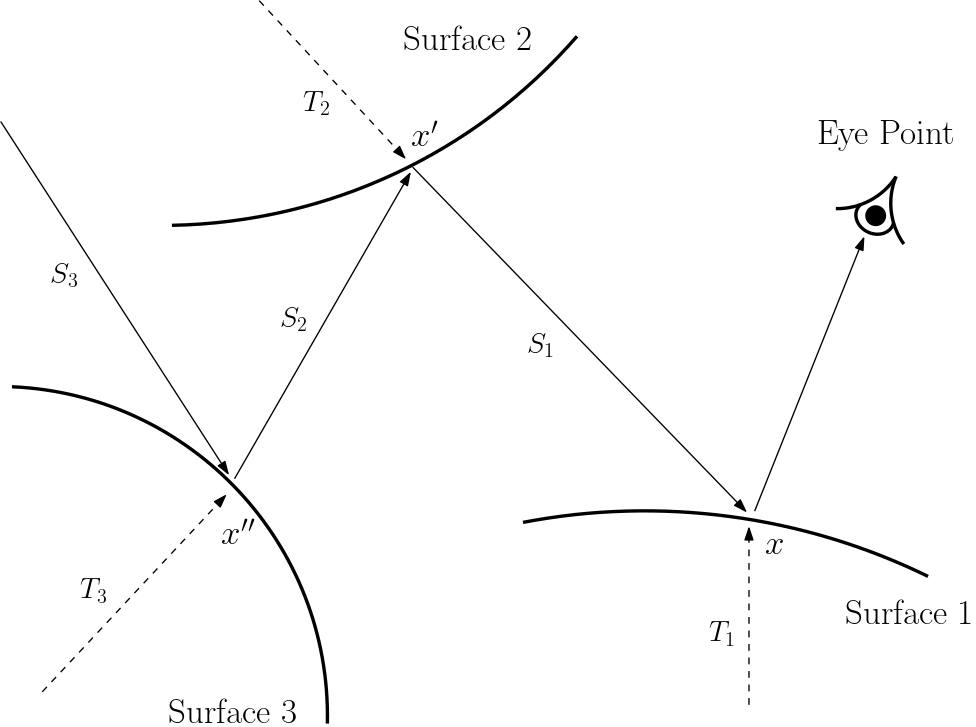
\includegraphics[width=.6\textwidth]{img/1 fundamentals/whitted_rays.png}\label{fig:whitted_rays}}
	\hfill
	\subfloat[Tree structure storing the individual reflection and transmission rays.]{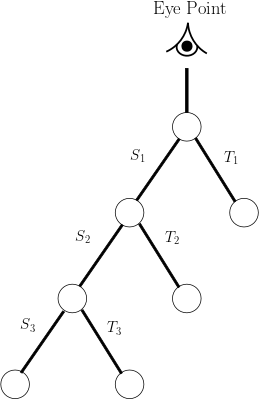
\includegraphics[width=.3\textwidth]{img/1 fundamentals/whitted_tree.png}\label{fig:whitted_tree}}
	\caption{Figures from the paper \citetitle{whitted1979improved} \cite{whitted1979improved}}
\end{figure}

This natural behavior is implemented in the following way. From the Eye Point, a ray is cast towards the virtual scene and a possible intersection point $x$ with the scene geometry is calculated. 


The transmission and specular component rays at that intersection point are then recursively calculated by Equation \ref{eq:whitted} and stored in a tree structure which is shown in Figure \ref{fig:whitted_tree}.  \todo{check check check}


Each node in this tree represents an intersection point and is furthermore associated with rays pointing towards \todo{rephrase} each light source in the scene, correlating to the $L_{j}$ terms in Equation \ref{eq:whitted}. If one of these light rays $L_{j}$ intersect scene geometry before it reaches light source $j$, the intersection point corresponding to the tree node in question is not illuminated by that particular light source and consequentially the contribution it to the reflection is not taken into consideration. To prevent a branch of the tree from growing infinitely large, it is truncated as soon as an attempt is made to access more storage than was made available for it. After such a tree is created, it is traversed recursively in order to calculate the light intensity at each node with Equation \ref{eq:whitted}, finally resulting in the calculation of the total light intensity that is reflected towards the $Eye Point$. Between two nodes, the intensity is attenuated according to a distance function between the intersection points associated with the node and the node's parent node. 
Such trees are created and traversed for every pixel of the image plane. This procedure allows for the convincing display of a variety of optical effects with the help of a single model.


\begin{figure}
	\centering
	\subfloat[Radiance is defined as the radiant flux emitted, received or reflected per solid angle $\partial\omega_{o}$ per unit projected area $\partial A$.]{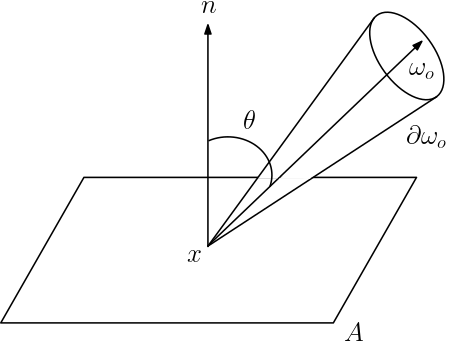
\includegraphics[width=.4\textwidth]{img/1 fundamentals/radiance.png}\label{fig:radiance}}
	\hfill
	\subfloat[The BRDF is a function defining how much light from the incoming direction$\omega_{i}$ is reflected towards the viewer along the outgoing direction $\omega_{o}$.]{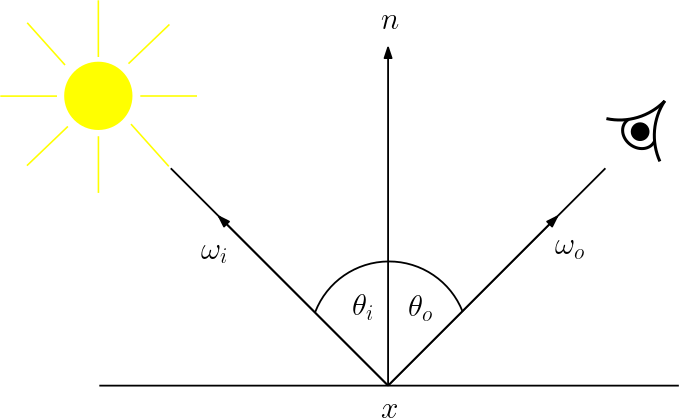
\includegraphics[width=.5\textwidth]{img/1 fundamentals/brdf.png}\label{fig:brdf}}
	\caption{Diagrams visualizing radiance (Figure \ref{fig:radiance}) and the BRDF (Figure \ref{fig:brdf}).}
\end{figure}

\todo{reformulate caption of radiance and brdf}

\subsection{The Rendering Equation}

In 1986, an integral equation was developed by Kajiya \cite{kajiya1986rendering}, that would describe the light transport

\begin{figure}
	\centering
	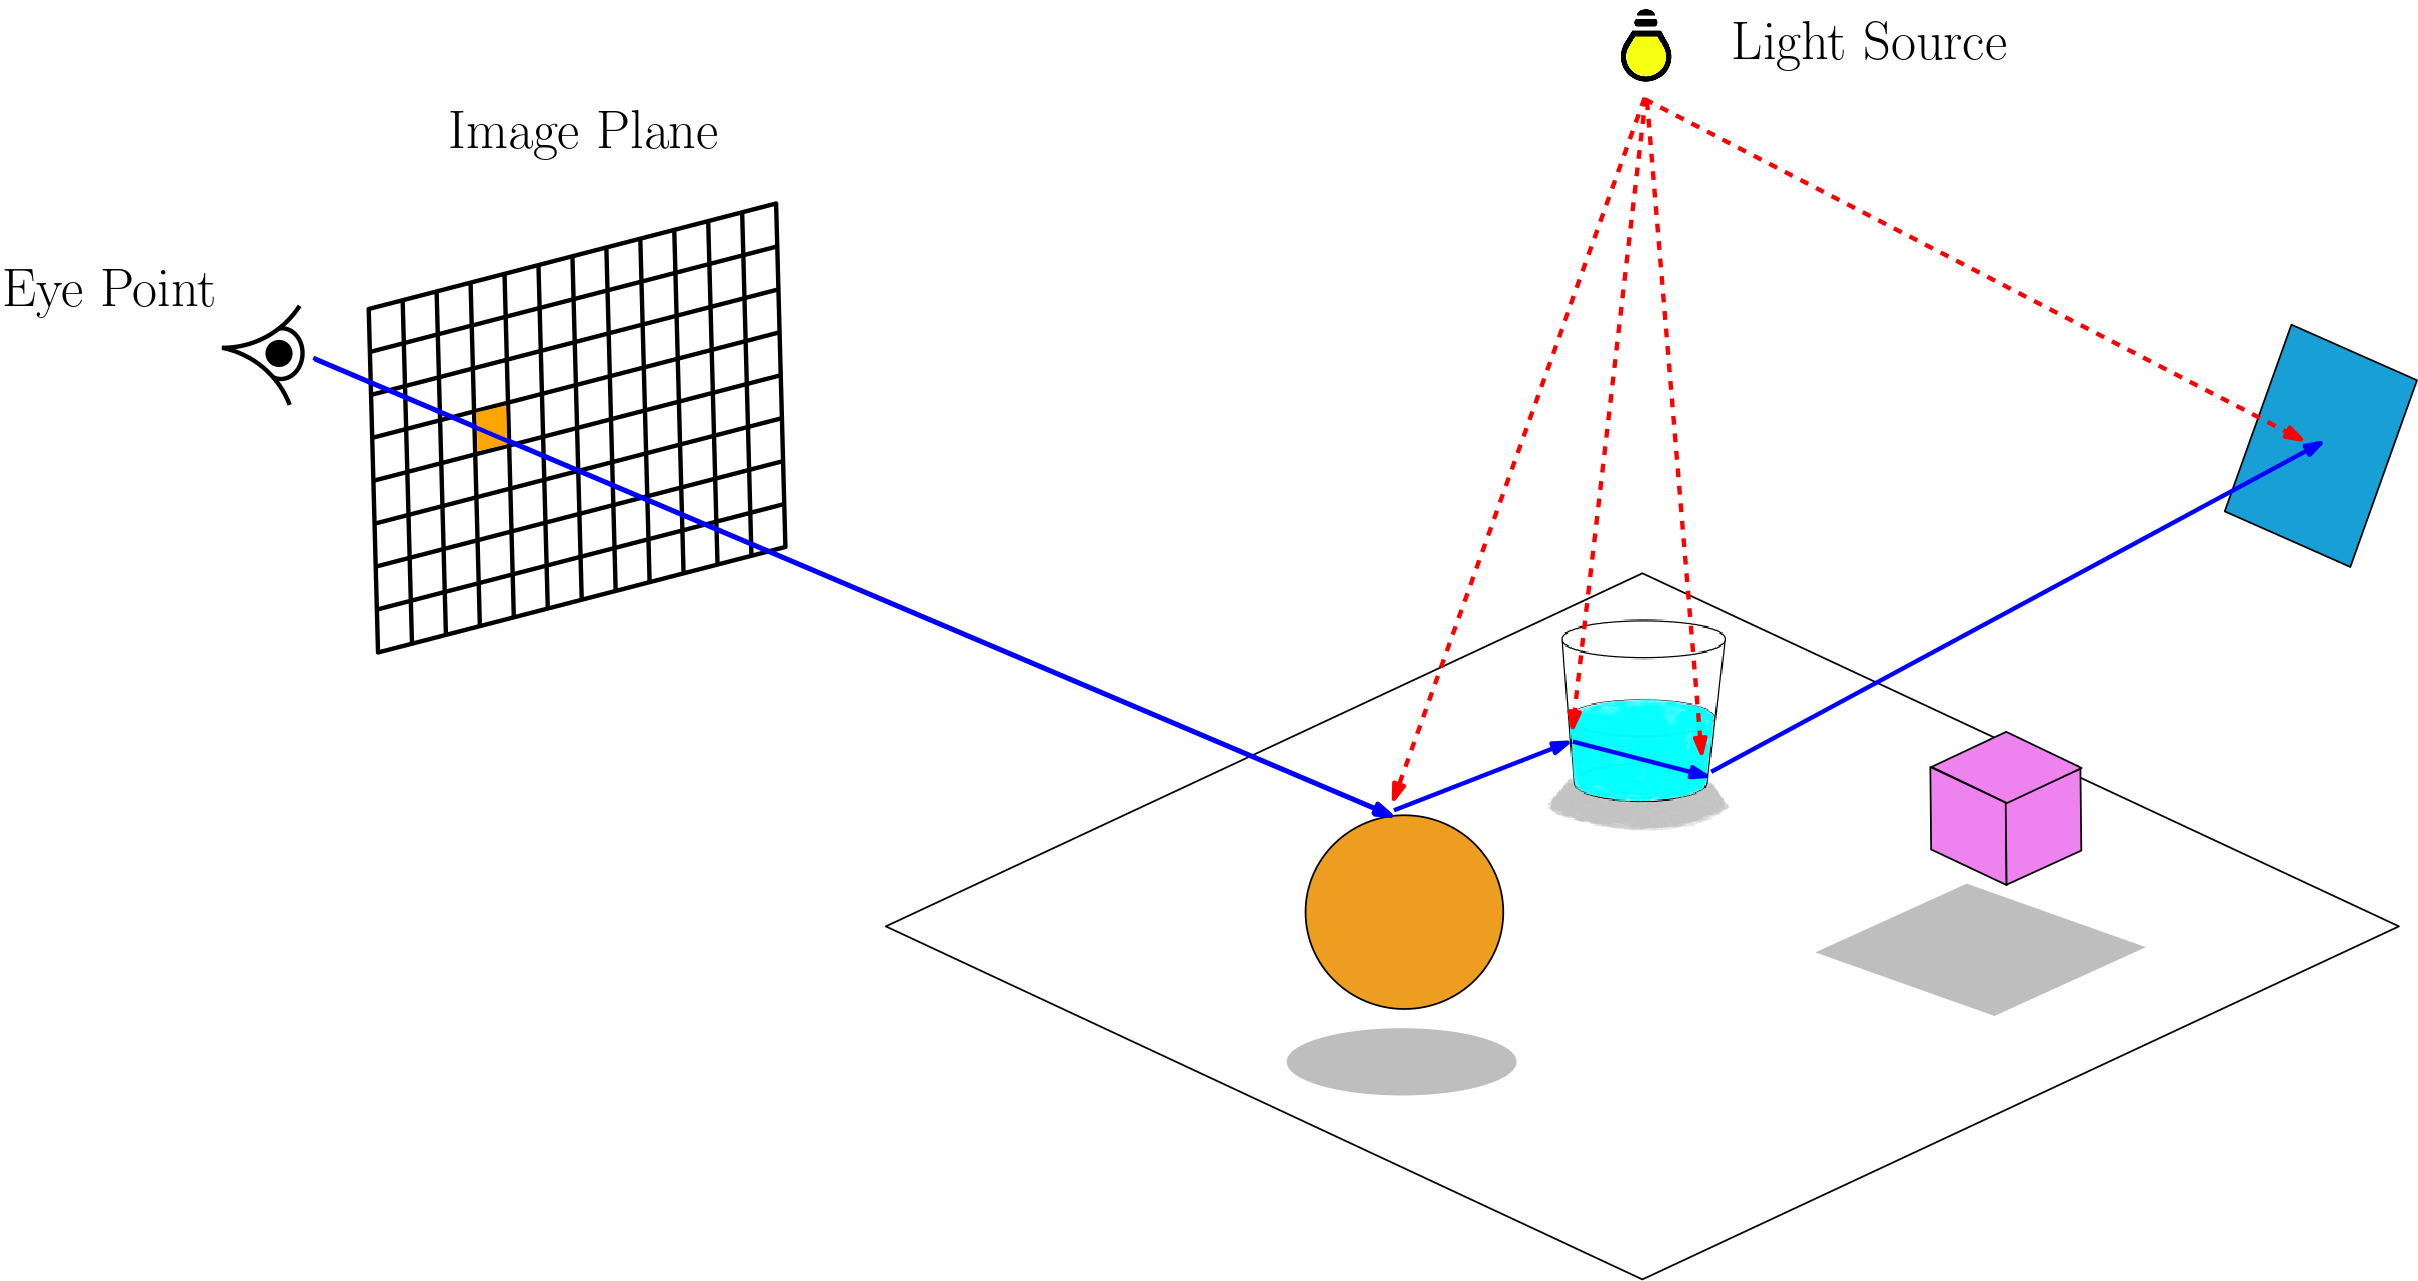
\includegraphics[width=1\linewidth]{img/1 fundamentals/path_tracing.png}
	\caption{Tracing a path for calculating global illumination.}
	\label{fig:pathtracing}
\end{figure}

\subsubsection{Derivation from the Definition of Radiance}

We define \emph{radiance} of a source, or informally "brightness", as the power per unit area $\partial A$ perpendicular to the ray in the direction $\omega_{o}$ and per unit solid angle that is propagated along it (see Figure \ref{fig:radiance}). This is described by the following equation:

\begin{equation}
L(\omega_{o}) = \frac{\partial^2\phi}{\partial\omega_{o}\partial A\cos\theta}
\end{equation}

\noindent where
\begin{description}
	\setlength\itemsep{0.05em}
	\item  $\omega_{o}$ is the outgoing direction
	\item  $\phi$ is flux or radiance per unit time
	\item  $A$ is the surface area, and
	\item  $\cos\theta$ a term for compensating Lambert's cosine law
\end{description}



\begin{equation}
BRDF(\omega_{i} \rightarrow \omega_{o}) = \frac{\partial L_{r}(\omega_{o})}{L_{i}(\omega_{i})\partial A\cos\theta}
\end{equation}

\noindent where
\begin{description}
	\setlength\itemsep{0.05em}
	\item  $L_r(\omega_{o})$ is the reflected radiance, and
	\item  $L_i(\omega_{i})$ is the incident radiance
\end{description}

\begin{equation}
L_{r}(\omega_{o}) = \int_{H(x)} L_{i}(\omega_{i})  BRDF(\omega_{i} \rightarrow \omega_{o}) \cos\theta\partial\omega_{i}
\end{equation}

\noindent where
\begin{description}
	\setlength\itemsep{0.05em}
	\item  $H(x)$ is a hemisphere over the interaction point $x$
\end{description}

\begin{equation}
L(\omega_{o}) = L_{e}(\omega_{o}) \int_{H(x)} L(ray(\omega_{i}, -\omega_{i})BRDF(\omega_{i} \rightarrow \omega_{o})\cos\theta\partial\omega_{i}
\end{equation}

\noindent where
\begin{description}
	\setlength\itemsep{0.05em}
	\item  $ray(\omega_{i}, -\omega_{i})$ is the recursive ray tracing function
\end{description}


\begin{figure}
	\centering
	\subfloat[]{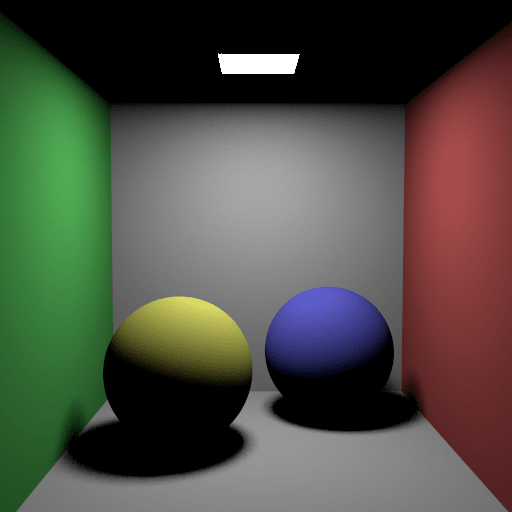
\includegraphics[width=.4\textwidth]{img/1 fundamentals/cb_direct.png}\label{fig:cb_local}}
	\hfill
	\subfloat[]{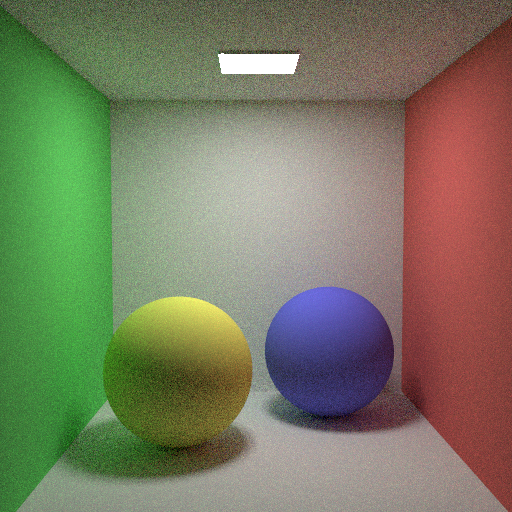
\includegraphics[width=.4\textwidth]{img/1 fundamentals/cb_global.png}\label{fig:cb_global}}
	\caption{The Cornell Box scene with local illumination (Figure \ref{fig:cb_local}) and global illumination (Figure \ref{fig:cb_global}).}
\end{figure}

\subsubsection{Monte Calo methods}
lalala


\section{Solid Representations in 3D Space}

A large part of the work of ray tracing algorithms is the calculation of intersection points between rays with scene geometry.
The way solid objects can be represented in the Euclidean space varies, thus does the testing for intersections with rays. The following section illustrates three types of solid representations in image synthesis environments, such as ART: Quadric surfaces, polygon meshes and constructive solid geometry.

\subsection{Quadric Surfaces}
\label{sec:quadrics}
Quadric surfaces are two dimensional surfaces in three dimensional Euclidean space, defined by quadric equations. Examples of these surfaces are spheres, cones, cylinders and paraboloids. The equations describing these shapes can be in implicit form, which have the pleasant property, that testing whether a point $p$ is located at the boundary of such a surface is easy. Generally speaking, implicit equations are relations of the form  $f(x_{0}, x_{1}, ..., x_{n}) = 0$ where $f$ is a function of multiple variables. Consider such a variable as a point $p$ in three dimensional space and evaluated by function $f$. An evaluation of $f$ will result in two possible outcomes: either $f(p) = 0$, which means $p$ is located on the surface of the shape, or  $f(p) \ne 0$, which means the opposite.
Due to this evaluation, quadrics are well suited for intersection testing during ray tracing. These quadratic function can furthermore be expressed in explicit form (sometimes referred to as parametric equation). An explicit equation is \todo{explain explicit function}.
In the following we will provide an example of an intersection calculation between a given unit sphere $S$ with radius $1$ and a given ray $R$. 

\begin{figure}[h]
	\centering
	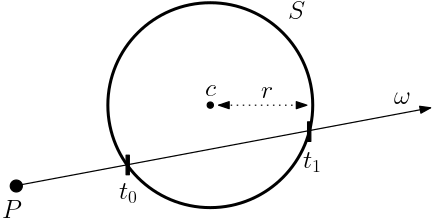
\includegraphics[width=.5\linewidth]{img/1 fundamentals/sphere_isect.png}
	\caption{Intersection between a sphere $S$ with its center point $c$ and radius $r$, and a ray with origin $P$ and direction $\omega$. We attempt to solve a quadradic equation in oder to obtain points $t_{0}$ and $t_{1}$. For reasons of simplicity, visualized in two dimensional space.} 
	\label{fig:sphere_isect}
\end{figure}

The sphere $S$ is implicitly defined by: 
\begin{equation} \label{eq:sphere}
S(x,y,z) = x^{2}+y^{2}+z^{2}-1 = 0
\end{equation}
The ray $R$ in its parametric form is defined by:
\begin{equation}\label{eq:ray}
R(t) = P + t\omega
\end{equation}

\noindent where
\begin{description}
	\setlength\itemsep{0.05em}
	\item  $P$ is the origin of ray $R$, a point in Euclidean space,
	\item  $t$ a scalar, and
	\item  $\omega$ the direction vector of $R$.
\end{description}

To obtain the two intersection points, the parametric equation defining $R$ is substituted into the implicit equation defining $S$
\begin{equation}\label{eq:substitution}
(P_{x}+t\omega_{x})^{2}+(P_{y}+t\omega_{y})^{2}+(P_{z}+t\omega_{z})^{2}-1 = 0
\end{equation}
and then, since all variables with the exception of $t$ are known, solved for $t$.
Once the two resulting values $t_{0}$ and $t_{1}$ are obtained, the two intersection points $I_{0}$ and $I_{1}$ can be expressed as $I_{0} = P + t_{0}\omega$, and respectively $I_{1} = P + t_{1}\omega$.

\subsection{Polygon Meshes}

Polygon meshes represent shapes as a composition of multiple, smaller polygons that are connected with each other. The higher the number of such polygons the mesh exhibits, the higher the accuracy of the approximation of the represented shape \todo{weird sentence.} The most common types of polygons used are triangles and quadrangles. An example of a representation of a shape with a triangle mesh can be seen in Figure \ref{fig:poly_mesh}. 

\begin{figure}
	\centering
	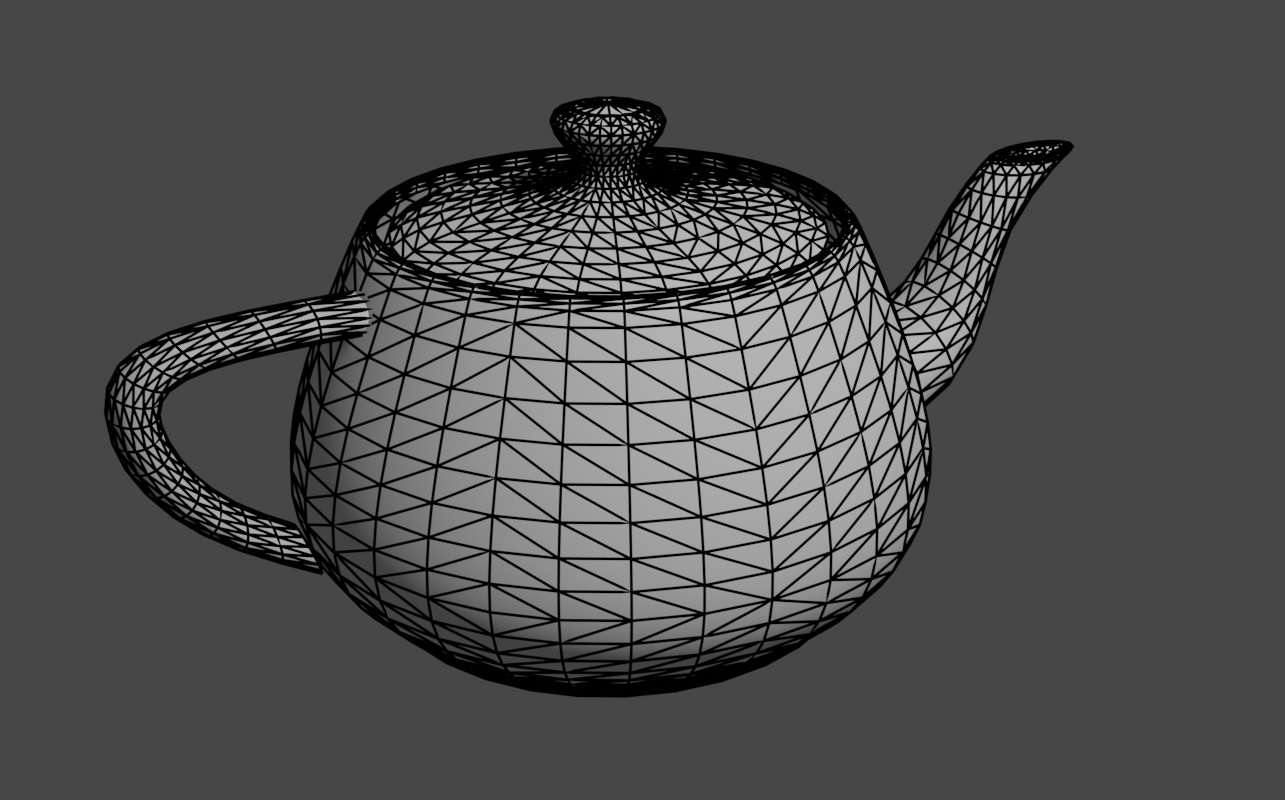
\includegraphics[width=.8\linewidth]{img/1 fundamentals/poly_mesh.png}
	\caption{Polygon mesh of the famous Utah Teapot, rendered with Blender \cite{blender2018}}
	\label{fig:poly_mesh}
\end{figure}

\subsection{Constructive Solid Geometry (CSG)}

The idea behind constructive solid geometry (CSG) modeling is the application of the boolean set operations to geometry primitive in order to create more complex geometries. The boolean set operators are union (logical \texttt{OR}), intersection (logical \texttt{AND}) and difference (denoted sometimes as \texttt{SUB}-operator). 
Primitives are usually quadric surfaces such as spheres, cones and cylinders. Figure \ref{fig:csg} shows the application of each boolean operator to two sphere primitives. Multiple of such set operations can be hierarchically ordered with the help of a binary tree structure, called the CSG-tree.   

\begin{figure} \label{csg}
	\centering
	\subfloat[Union of two spheres (\texttt{OR} operator).]{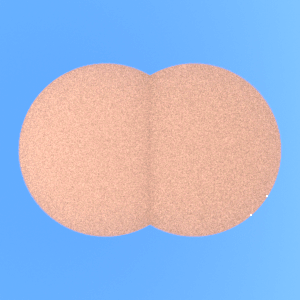
\includegraphics[width=.3\textwidth]{img/1 fundamentals/or.png}\label{fig:csg_or}}
	\hfill
	\subfloat[Intersection of two spheres (\texttt{AND} operator).]{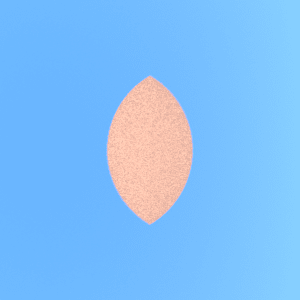
\includegraphics[width=.3\textwidth]{img/1 fundamentals/and.png}\label{fig:csg_and}}
	\hfill
	\subfloat[Left sphere with the right sphere "subtracted" from it (\texttt{SUB} operator).]{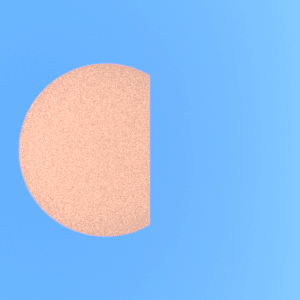
\includegraphics[width=.3\textwidth]{img/1 fundamentals/sub.png}\label{fig:csg_sub}}
	\caption{Boolean operators Union (\ref{fig:csg_or}), Intersection (\ref{fig:csg_and}) and Difference (\ref{fig:csg_sub}) applied to two sphere objects.}
\end{figure}

One example of such CSG tree is provided in Figure \ref{fig:csg_tree}. Its leafs are associated with the geometry primitives, the nodes with the set operations. Due to the possibility that two primitives can face being translated, rotated or scaled before a boolean operator is applied to them, edges of the tree is associated with transformation information (this is denoted in the figure with the matrix icon). The transformation corresponding to an edge between a node and a node's parent can be "empty", meaning that it has no effect on the primitive represented by that node.  

\begin{figure}
	\centering
	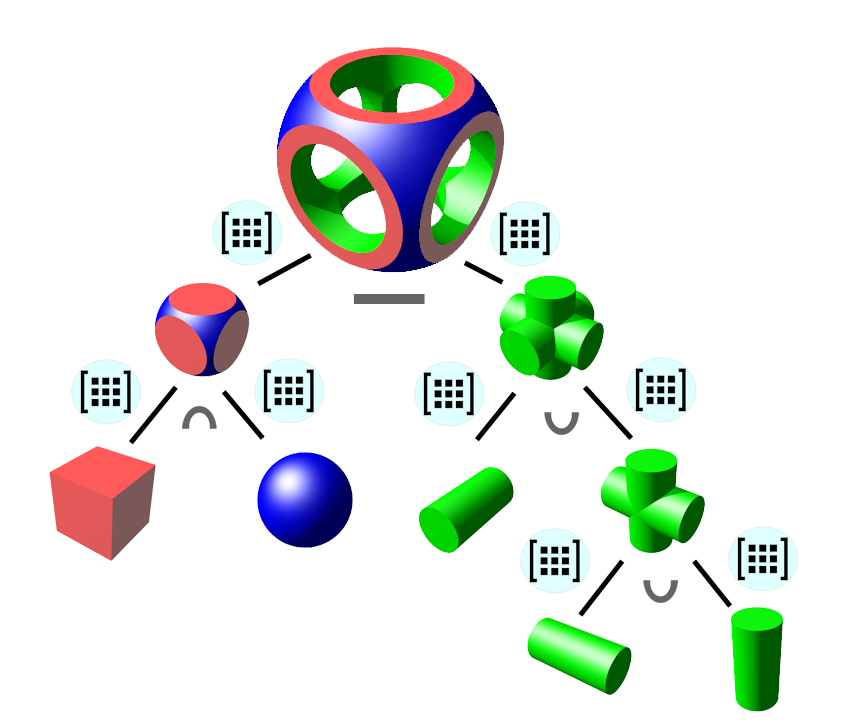
\includegraphics[width=.9\linewidth]{img/1 fundamentals/csg_tree.png}
	\caption{Visualization of a CSG tree hierarchy, originally created by \cite{csgtree} and updated
	with a matrix icon symbolizing affine transformations of geometries.}
	\label{fig:csg_tree}
\end{figure}

The intersection calculation for a given ray during the ray tracing process is straightforward: 
All the primitives associated to the leafs of the CSG tree are tested for intersection. If an intersection test has a positive result, usually two intersection points are calculated: one  with one primitive is found, one point when the ray enters the primitive and one point when it exits it (there is the edge case that there exists infinitely many intersection points between a ray and a primitive when the ray is tangent to the primitive, however, this is seldom the case and can be safely ignored). Then the CSG tree is traversed bottom up and each time an interior node representing a boolean set operator is encountered, the intersection points of the ray with the primitives associated with the child nodes are evaluated and re-arranged. For example, when considering the \texttt{OR} operator in Figure \ref{fig:csg_or}, and imagining a single ray would intersect both spheres, there would be four intersection points: One entering the first sphere, followed by one entering the second sphere, then one exiting the first sphere, and finally one intersection point exiting the second sphere. The \text{OR} operator would treat the two spheres as one single object and therefore discard the inner intersection points. Similarly, the \text{AND} operator in Figure \ref{fig:csg_and} would discard the intersection of a sphere that is not in the interior of the other sphere. And finally, the \text{SUB} operator in Figure \ref{fig:csg_sub} discards every intersection point on the sphere on the right, which is "subtracted" from the sphere on the left.

The representation of CSG offers one significant advantage: Complex geometry can be expressed via the composition of a manageable amount of primitive shapes, as opposed to large numbers of polygons in a polygon mesh. Because testing whether a point lies inside or outside a primitive is easy, as noted in Section \ref{sec:quadrics}, and since compared to polygon meshes only a small amount of primitives exist, the number of intersection tests in each render pass is comparatively low.

Although the CSG modeling technique is several years old (being introduced by \cite{roth1982ray}), it is still used in practice today, e.g. for computer-aided design.

% new section
\section{Common ray acceleration data structures}
The computational cost associated with ray tracing algorithms has always been regarded as a "necessary evil" one has to face when desiring highly realistic images. An often cited fact is Whitted's observation, that, for complex scenes, 95 percent of the time used by the algorithm is spend on intersection calculations \cite[p 349]{whitted1979improved}. The image displayed in figure \ref{fig:rendering_eq}, was rendered with a resolution of 512 by 512 pixels and with 40 paths per pixel on an IBM 3081 machine consumed during 1221 minutes \cite[p 149]{kajiya1986rendering}. 

It was a logical consequence, that, over time, new ideas were introduced for accelerating the ray tracing process, mostly by minimizing the number of intersection tests. Nowadays, there exist various ray acceleration structures. In the following, two of these structures are that are commonly used, namely bounding volume hierarchies and binary space partitioning trees are introduced.

\subsection{Bounding volume hierarchy}

\subsection{Binary space partitioning}


\section{Intel\textregistered's Embree Framework}
Embree is a high performance rendering framework, consisting of a collection of kernels and data structures suited for the communication with [insert hardware types]. The latest version of Embree at the time of writing this thesis is 3.13.0.